\documentclass[notitlepage]{revtex4-1}

\usepackage{amsmath}

\usepackage{bm}

\usepackage{physics}

\usepackage{algorithm}
\usepackage{algpseudocode}

\usepackage{graphicx}
\usepackage{subcaption}
\usepackage{epstopdf}
\graphicspath{{img/}}

\everymath{\displaystyle}

\begin{document}

\title{Learning dynamics of Restricted Boltzmann Machines}

\author{Giancarlo Fissore}
\email{giancarlo.fissore@gmail.com}
\affiliation{Laboratoire de Recherche en Informatique, TAO - INRIA, Universit\'e Paris-Sud, Bat. 660, 91190 Gif-sur-Yvette, France.}

\date{28 June 2017}

\begin{abstract}
Restricted Boltzmann Machines (RBMs) are elementary generative models that have been shown to be effective on their own or as building blocks for deep architectures. Despite their relative simplicity, however, a deep theoretical understanding of their functioning is missing and we try to improve on this situation by analysing the learning dynamics of such model. First, we compare a new physics-inspired training algorithm to the classical persistent contrastive divergence method, finding that the classical strategy is slightly preferable. However, the minor differences that we observed do not impact the learning dynamics and leveraging the tools of statistical physics we show that a theoretical framework to study RBMs can be identified. In particular, mean-field methods are shown to provide a good characterization for the linear regime in which RBMs are found to operate at the beginning of the training. In this regime, it is shown that the parameters of the model are learnt in such a way to reproduce the singular value decomposition of the training data. Moreover, looking at the dynamical evolution of the model's parameters it is shown how the learning dynamics are initially fast and then slow down, and a cutoff in the parameters is found which we interpret as a signal to stop the learning. Finally, a basic statistical characterization of the parameters for a trained RBM is highlighted.
\end{abstract}

\maketitle

\section*{Introduction}
In the last years progresses in machine learning have led to spectacular applications in many fields such as computer vision, image classification and speech recognition, giving results that were believed to be decades away \cite{go}. While the practical applications are of tangible impact, however, our theoretical understanding of the models in use is poor. From this point of view, unsupervised learning presents specific challenges different from those of supervised learning \cite{foundations}, the former being the problem of automatically extracting structure from data while the latter refers to the ability to learn a rule that maps data to their appropriate labels. What we are interested in is the matter of automatically constructing generative models from a dataset, a problem which arises in the context of unsupervised learning.

While generative models in use can be arbitrarily complex, not even the most elementary models such as RBMs, a simple neural network with only one hidden layer, are well understood. Historically, the theoretical foundations of neural networks have been grounded in statistical physics \cite{hist1}\cite{hist2} and in this work we show the effectiveness of this approach applied to the RBM model.

After a brief overview on the RBM model, we present a recently proposed training algorithm based on statistical physics \cite{tap_train}\cite{tap}. A comparison to classical Monte Carlo based algorithms is then given, showing the substantial equivalence of the methods. This preliminary analysis paves the ground for a careful examination of the dynamics of learning, which are found to be independent on the specific training procedure used. The RBM is then studied in the linear regime, where mean-field theory from statistical physics helps in identifying the Singular Value Decomposition (SVD) of the RBM parameters as the SVD of the training data.
 %finding a relation between the singular value decomposition (SVD) of the training data and the SVD of the RBM parameters.
On this basis, the analysis of the dynamical evolution of the SVD of the RBM parameters produces a detailed picture of how the structure of the training data is embedded into the model. This increases our understanding of the learning process and gives some clear insights to understand when the learning has come to an end, improving on current criteria based on flatness of a likelihood function and subjective quality of generated samples.

Finally, the SVD analysis let us differentiate the trained RBM parameters in a set of random parameters that represent noise and can be discarded and a set of structured non-random parameters. This is a first advance in an attempt to determine the proper statistical ensemble of the RBM model, in order to improve current theoretical treatments which are based on the approximation that parameters are random and independent \cite{monasson}.

\section{Training Restricted Boltzmann Machines} \label{training}

\subsection{Definition of the model}

A RBM is a model for neural networks which basically consists in a bipartite graph with a layer of hidden units \(h_j\) and a layer of visible units \(v_i\). The units in one layer are not connected among them but are connected to all the units in the other layer, as shown in fig. \ref{fig:rbm}. We restrict our treatment to the case of binary units \(h_i,v_i = 0,1\). Drawing a comparison between RBMs and spin models in statistical physics, we can define the following \textit{energy function}

\begin{equation}
E(\textbf{h},\textbf{v}) = - \sum_i a_i v_i - \sum_j b_j h_j - \sum_{i,j} v_i w_{ij} h_j
\label{eq:ef}
\end{equation}

where \(a_i\) and \(b_i\) are \textit{external fields} acting respectively on the visible and hidden units. The probability of a certain configuration is then given by the Boltzmann measure (taking \(\beta = 1\))

\begin{equation}
P(\textbf{h},\textbf{v}) = \frac{e^{-E(\textbf{h},\textbf{v})}}{Z}
\end{equation}

where \( \textstyle Z = \sum_{\textbf{h},\textbf{v}} e^{-E(\textbf{h},\textbf{v})}\) is the \textit{partition function}. The probabilities of activations for visible and hidden units can be simply computed to be (given the independence of units in the same layer)

\begin{align}
P(v_i = 1 | \textbf{h}) &  = \frac{1}{1+e^{-a_i - \sum_{j} w_{ij} h_j}} \nonumber \\
& = sigm \left(a_i + \sum_{j} w_{ij} h_j \right)
\label{eq:act_vis}
\end{align}

\begin{align}
P(h_j = 1 | \textbf{v}) & = \frac{1}{1+e^{b_j + \sum_i w_{ij} v_i}} \nonumber \\
& = sigm \left(b_j + \sum_i w_{ij} v_i \right)
\label{eq:act_hid}
\end{align}

\begin{figure}
  \centering
  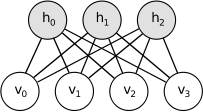
\includegraphics{rbm.png}
  \caption{bipartite structure of a RBM}
  \label{fig:rbm}
\end{figure}

We see that the usual neuron activation function (the sigmoid function, which we indicated by \(sigm\)) comes out naturally by choosing binary units \(h_j,v_i = 0,1\). Moreover, we can now understand the importance of the external fields: they drive the activation of a certain unit by setting a threshold that has to be overcome by the opposite layer through the couplings \(w_{ij}\).

What we are interested in is the probability for the visible units, which is the layer we use to represent data. It can be easily defined as

\begin{align}
P(\textbf{v}) &  = \sum_{\textbf{h}} P(\textbf{h},\textbf{v}) \nonumber \\
& = \frac{e^{-F_c(\textbf{v})}}{Z}, \quad Z = \sum_{\textbf{v}} e^{-F_c(\textbf{v})}
\label{eq:p_model}
\end{align}

where, further exploiting the parallel with spin models, we have introduced the \textit{clamped free energy}

\begin{align}
F_c(\textbf{v}) & = -\log \sum_{\textbf{h}} e^{-E(\textbf{h},\textbf{v})} \nonumber \\
& = -\sum_i a_i v_i -\sum_j \log \left( 1 +  e^{\left( b_j + \sum_i w_{ij} v_i \right)} \right)
\end{align}

To use the RBM as a generative model, we want to maximize \(P(\textbf{v}\)) for the samples belonging to the training set. This is done by performing gradient ascent over the log-likelihood \(\log P(\textbf{v})\), whose derivative with respect to the weights can be computed to be

\begin{equation}
\frac{\partial \log P(\textbf{v})}{\partial w_{ij}} = \langle v_i P(h_j = 1 | \mathbf{v}) \rangle_{data} - \langle v_i h_j \rangle_{model}
\label{eq:opt}
\end{equation}

where \(\langle \cdot \rangle_{data}\) denotes an average over the empirical distribution of the training set (\( \textstyle P_{data}(\mathbf{v}) = \frac{1}{N} \sum_{\mathbf{v}_n \in data} \delta (\mathbf{v} - \mathbf{v}_n ) \)) and 
\(\langle \cdot \rangle_{model}\) denotes the average over the distribution \eqref{eq:p_model}. Introducing the \textit{learning rate} \(\alpha \) (as a parameter for gradient ascent) we obtain an update rule for the weights matrix

\begin{equation}
\Delta \mathbf{W} = \alpha \left( \langle \mathbf{v h}^T \rangle_{data} - \langle \mathbf{v h}^T \rangle_{model} \right)
\label{eq:w_up}
\end{equation}

In the same way we can get the update rules for the external fields

\begin{equation}
\label{eq:a_up}
\Delta \mathbf{a} &= \alpha \left( \mathbf{v}_{data} - \mathbf{v}_{model} \right)
\end{equation}
\begin{equation}
\label{eq:b_up}
\Delta \mathbf{b} &= \alpha \left( \mathbf{h}_{data} - \mathbf{h}_{model} \right)
\end{equation}

Given the update rules, the training consists in actually performing the gradient ascent. Once this is done, it is possible to sample the equilibrium configurations of the RBM to obtain samples which are generated according to the probability distribution of the training data. Unfortunately, the average over the model distribution \(\textstyle \langle \cdot \rangle_{model}\) is intractable as such term is exponential in the number of visible units. Approximations are then necessary to train and sample from a RBM; in particular Monte Carlo based algorithms are generally employed, such as \textit{k-steps contrastive divergence} (CDk) \cite{Hinton_CD}  and \textit{persistent contrastive divergence} (PCD) \cite{PCD}. Approximate algorithms based on mean-field methods from statistical physics have also been employed, but showing results of inferior quality with respect to CDk-PCD \cite{PCD}. Recently, however, a new algorithm based on mean-field has been proposed \cite{tap_train}, showing results comparable to the usual Monte Carlo based methods. An overview of this novel algorithm and an analysis of its performance is given in the next sections.

\subsection{Training via extended mean-field} \label{sec:emf}
We have already drawn attention to the similarities between the RBM model and spin models in statistical physics. In particular, the energy function \eqref{eq:ef} corresponds to the hamiltonian of the spin glass Sherrington-Kirkpatrick (SK) model \cite{SK} and this makes it possible to take advantage of well established results in spin glass theory to obtain a valid approximation to the intractable term in the update rule \eqref{eq:w_up}. In fact, looking back at the log-likelihood we can express it as

\begin{align}
\log P(\mathbf{v}) &= \log \frac{e^{-F_c(\mathbf{v})}}{Z} \\ \nonumber
&= -F_c(\mathbf{v}) - F
\end{align}

where \( \textstyle F = - \log Z \) is the \textit{free energy} of the SK model and it corresponds to the intractable term. Introducing the inverse temperature \(\beta\) we can write the Boltzmann measure of the SK model where the role of the spins is played by the units of the RBM and the separation between visible and hidden layers is retained only to make the connection between the two models clear

\begin{equation}
P(\textbf{h},\textbf{v}) = \frac{e^{- \beta E(\textbf{h},\textbf{v})}}{Z}
\end{equation}

By means of a high-temperature expansion (\(\beta \to 0\)) \cite{ht_exp} it is then possible to obtain the Thouless-Anderson-Palmer (TAP) expression for the free energy \cite{TAP} that, in the context of a RBM and truncated at second order, can be written as

\begin{align}
F_{TAP}(\mathbf{m}^v,\mathbf{m}^h) = &+ S(\mathbf{m}^v) + S(\mathbf{m}^h) \nonumber \\
&- \sum_i a_i m_i^v - \sum_j b_j m_j^h - \sum_{i,j} w_{ij} m_i^v m_j^h \nonumber \\
&+ \sum_{i,j} \frac{w_{ij}^2}{2} \left( m_i^v - {m_i^v}^2 \right) \left(m_j^v - {m_j^h}^2 \right) \label{eq:f_tap}
\end{align}

with \( \textstyle S(\mathbf{m}) = - \sum_i \left[ m_i \log m_i + (1 - m_i) \log (1 - m_i) \right] \).

We note that \(F_{TAP}\) is an \textit{effective free energy} expressed in terms of the magnetizations \(\mathbf{m}^v, \mathbf{m}^h\), given by eq. \eqref{eq:act_vis},\eqref{eq:act_hid}. Its minimization gives a valid approximation to the free energy \(F\)

\begin{equation}
F \simeq F_{TAP}(\mathbf{\tilde{m}}^v, \mathbf{\tilde{m}}^h), \qquad \left. \frac{dF_{TAP}}{d \mathbf{m}} \right\rvert_{\mathbf{\tilde{m}}^v, \mathbf{\tilde{m}}^h} = 0
\label{eq:f_approx}
\end{equation}

To obtain \(\mathbf{\tilde{m}}^v, \mathbf{\tilde{m}}^h\) it is then necessary to extremise \eqref{eq:f_tap} to obtain the following coupled equations

\begin{align}
m_i^v \simeq sigm \left\{ a_i + \sum_j \left[ w_{ij} m_j^h - w_{ij} \left( m_i^v - \frac{1}{2} \right) \left( m_j^h - {m_j^h}^2 \right) \right] \right\} \label{eq:tap_vis} \\
m_j^h \simeq sigm \left\{ b_j + \sum_i \left[ w_{ij} m_i^v - w_{ij} \left( m_j^h - \frac{1}{2} \right) \left( m_i^v - {m_i^v}^2 \right) \right] \right\} \label{eq:tap_hid}
\end{align}

that can be solved by iteration \cite{conv}. Finally, given the approximation to the free energy \eqref{eq:f_approx}, the optimization problem over the log-likelihood \eqref{eq:opt} is greatly simplified: the average over the training samples \(\textstyle \langle \cdot \rangle_{data}\) is unchanged while the intractable average over the model distribution \(\textstyle \langle \cdot \rangle_{model}\) is substituted by the maximization of \eqref{eq:f_approx}, giving

\begin{equation}
\Delta \mathbf{W} = \alpha \left( \langle \mathbf{v h}^T \rangle_{data} - \frac{\partial F_{TAP}(\mathbf{\tilde{m}}^v, \mathbf{\tilde{m}}^h)}{\partial w_{ij}} \right)
\label{eq:w_up_tap}
\end{equation}

Summarizing, the training procedure based on TAP approximation is reported in the following algorithm.

\begin{algorithm}[H]
\caption{Extended mean-field training}\label{alg:tap}
\begin{algorithmic}[1]
\State \textbf{Data:} a training set of N data vectors
\State Randomly initialize the weights matrix \textbf{W}
\For{t = 0 to T (\# of epochs)}
  \ForAll{vectors in the training set}
    \State initialize  \(m_j^h=P(h_j|\mathbf{v}),m_i^v=P(v_i|\mathbf{h})\)
    \State iterate TAP equation \eqref{eq:tap_vis},\eqref{eq:tap_hid} to convergence to obtain \(\tilde{\mathbf{m}}^v,\tilde{\mathbf{m}}^h\)
    \State update \(\mathbf{W}\) with eq. \eqref{eq:w_up_tap}
  \EndFor
\EndFor
\end{algorithmic}
\end{algorithm}

We conclude by noting how the introduction of the inverse temperature \(\beta\) is just a formal passage; in the context of a RBM we keep \(\beta = 1\) and the high-temperature expansion is substituted by a weak-couplings expansion, under the assumption that the weights \(w_{ij}\) are small enough (this assumption is verified in next sections). The variance of the weights matrix can then serve as an \textit{effective inverse temperature} \cite{monasson}, giving

\begin{equation}
T_{eff} = \frac{1}{Var(\mathbf{W})}
\label{eq:t_eff}
\end{equation}

\subsection{Analysis of the learning}
To assess the performance of the extended mean-field (EMF) training described in section \ref{sec:emf} we have trained a RBM using both PCD and EMF and compared the outcomes, implementing both algorithms following the guidelines given in \cite{Hinton_guide}.

The dataset we used is the MNIST database \cite{mnist}, a set of \(70000\) handwritten digits whose samples consist in \(28 \times 28\) pixels centered and size-normalized images. The first \(60000\) samples are used for training the RBM while the remaining \(10000\) samples constitute the test set, that is used to validate the training and monitoring for overfitting. Examples of the MNIST samples are shown in fig. \ref{fig:samples_mnist}.

Drawing samples from the trained distribution \(P(\mathbf{v},\mathbf{h})\) is done by performing Gibbs sampling \cite{gibbs}, which basically consists in running a Markov chain to convergence. In the context of a RBM, as there are no links among units in the same layer, we can perform the sampling in blocks: starting from a visible configuration the conditional probability of the hidden layer is computed using \eqref{eq:act_hid} and this makes it possible to compute the conditional probability of the visible layer, starting a loop that if iterated long enough is guaranteed to produce samples approximating the joint probability distribution of all the variables. The sampling algorithm is reported below for clarity.

\begin{algorithm}[H]
\caption{Gibbs sampling}\label{alg:gibbs}
\begin{algorithmic}[1]
\State \textbf{Init:} take a random configuration \(\mathbf{v}\)
\For{i=0 to k}
  \State \( \mathbf{h} = P(\mathbf{h}|\mathbf{v}) \)
  \State \( \mathbf{v} = P(\mathbf{v}|\mathbf{h}) \)
\EndFor
\State Set \(v_i = 1\) with probability \(P(v_i = 1|\mathbf{h})\)
\end{algorithmic}
\end{algorithm}

The results of the training are affected by many parameters, that we have set empirically and in accordance to \cite{PCD}\cite{tap_train}. A summary for our choices is given below:

\begin{itemize}
  \item \(\sigma_v = 0.01\): this is the variance for the initialization of the weights \(\mathbf{W}\) as a gaussian random matrix. This value is agreed to work well and it fits our requirement of having small weights in order to perform the weak couplings expansion
  \item \(\alpha = 0.01\): a larger learning rate would speed up the training but making the RBM initially learn a bad model of the data that is then difficult to refine during succeeding epochs. A small learning rate is then preferred to obtain a good generative model.
  \item \(d = 784\): number of visible units, set in accordance to the dimensionality of MNIST images (\(28 \times 28\)).
  \item \(p = 500\): number of hidden units, set in accordance to other works on the MNIST database. A too small number would not make it possible to accurately represent all the characteristics of the training data while a too big number would result in a redundant increase in the complexity of the model.
  \item batch size \(m = 100\): training data are not processed one by one but in batches, so that the operations can be vectorized to speed up the learning. The higher the batch size, the more efficient the learning. Lower batch sizes, however, are found to give better generative models and in our case the chosen value is a good trade-off.
  \item \( k = 5 \): number of Gibbs sampling steps used for PCD learning. For EMF, we recall that no Gibbs sampling steps are necessary during training.
\end{itemize}

\begin{figure}
  \centering
  \begin{subfigure}{.25\linewidth}
    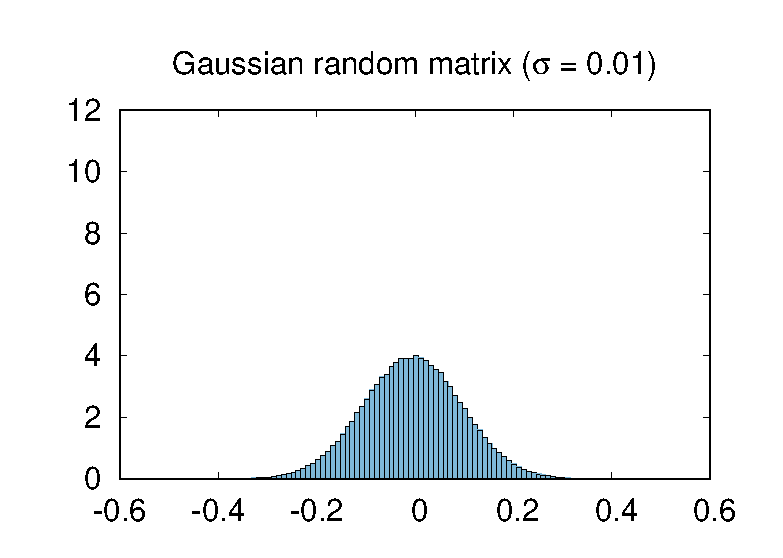
\includegraphics[width=\linewidth]{w_init.eps}
    \caption{}
    \label{fig:w_init}
  \end{subfigure}
  \begin{subfigure}{.25\linewidth}
    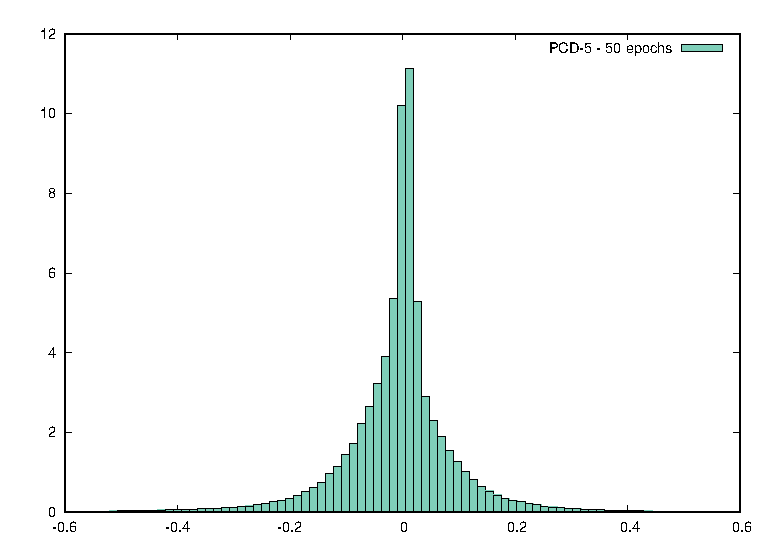
\includegraphics[width=\linewidth]{w_pcd5_50.eps}
    \caption{}
    \label{fig:w_pcd5_50}
  \end{subfigure}
  \begin{subfigure}{.25\linewidth}
    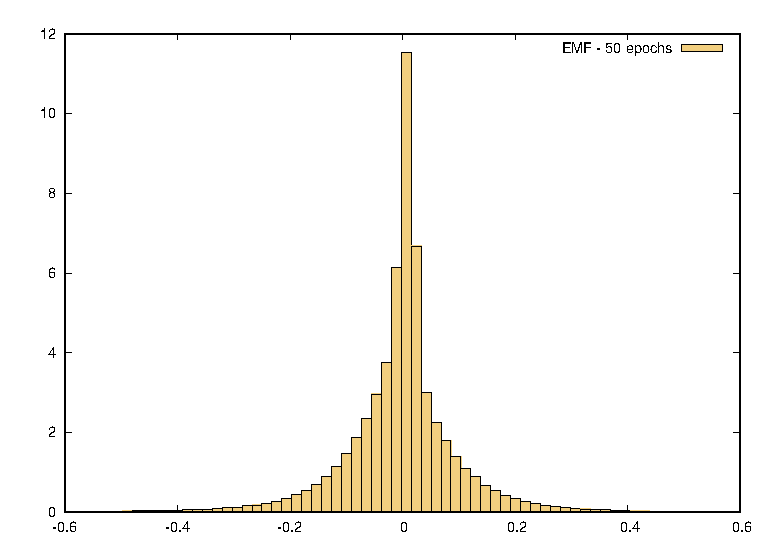
\includegraphics[width=\linewidth]{w_tap20_50.eps}
    \caption{}
    \label{fig:w_tap20_50}
  \end{subfigure}\par\medskip
  \begin{subfigure}{.25\linewidth}
    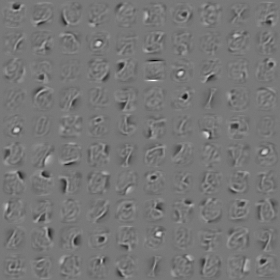
\includegraphics[width=\linewidth]{features_pcd.png}
    \caption{}
    \label{fig:features_pcd}
  \end{subfigure}
  \begin{subfigure}{.25\linewidth}
    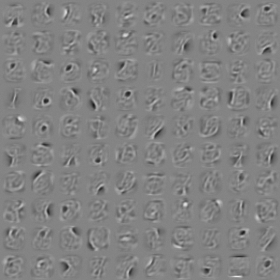
\includegraphics[width=\linewidth]{features_tap.png}
    \caption{} 
    \label{fig:features_tap}
  \end{subfigure}
  \begin{subfigure}{.25\linewidth}
  	\begin{subfigure}{.5\linewidth}
  		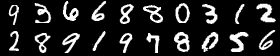
\includegraphics[width=\linewidth]{samples.png}
        \caption{} 
        \label{fig:samples_mnist}
  	\end{subfigure}
  	\begin{subfigure}{.5\linewidth}
  		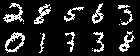
\includegraphics[width=\linewidth]{samples_pcd.png}
        \caption{} 
        \label{fig:samples_pcd}
  	\end{subfigure}
  	\begin{subfigure}{.5\linewidth}
  		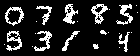
\includegraphics[width=\linewidth]{samples_tap.png}
        \caption{} 
        \label{fig:samples_tap}
  	\end{subfigure}
  \end{subfigure}
  
 \caption{\textbf{(a)} Weights distribution before training (gaussian). \textbf{(b)-(c)} Weights distribution after a 50 epochs training for PCD and EMF: the two distributions are very similar, peaked around zero and showing fatter tails with respect to (a). \textbf{(d)-(e)} Hidden features obtained with PCD and EMF: no qualitative difference is observed between the two. \textbf{(f)} Samples taken from MNIST dataset. \textbf{(g)-(h)} Samples obtained respectively with PCD and EMF. We can see how the EMF training generates spurious states.}
\end{figure}

The comparison between PCD and EMF is performed by looking at the weights distribution, the generated hidden features and the samples generated by the trained RBM.

The weights distribution after training is shown in fig. \ref{fig:w_pcd5_50}-\ref{fig:w_tap20_50}. For both PCD and EMF the initial gaussian distribution is shrinked to a more peaked distribution around zero, but the tails of the distribution get fatter. This results in an increase in the variance of \(\mathbf{W}\) and a corresponding decrease in the effective temperature \eqref{eq:t_eff}, suggesting that the weak couplings expansion is not justified anymore in late phases of the training. This, in turn, indicates how the EMF training could eventually break down after a long enough training, while PCD is not affected by this problem. However, the effective temperature does not decrease indefinitely; after a small but substantial number of epochs (circa \(20\) in our case) it converges to a low value.

In fig. \ref{fig:features_pcd}-\ref{fig:features_tap}, instead, the hidden features generated by the RBM are shown. Each consists in the activation pattern of the visible layer driven by a single hidden unit, and their ensemble corresponds to the strokes by which the samples generated by the RBM are composed \cite{monasson}. No qualitative difference is found among PCD and EMF features, and this serves as a first hint that the charachterization of a trained RBM is independent from the training procedure. 

The most significant comparison between the two methods is given by looking at the samples generated by the trained models, shown in fig. \ref{fig:samples_pcd}-\ref{fig:samples_tap}. Both methods generate good models of the training data, but we can see that for EMF some samples are not resembling real digits. This is an artifact of the learning which is found also for PCD, even if it is more evident for EMF; an investigation on the matter is given in \cite{leroy}\cite{tap}.

As a conclusion, we see that PCD and EMF training give comparable results, apart from the spurious states generated by EMF. On this basis, next sections are devoted to a careful analysis of the learning procedure. As for the features, all results and observations that we will show are equally valid for both PCD and EMF, giving further confirmation that the learning dynamics are independent on the details of the learning algorithm. The strength of EMF, however, is the ability to provide a theoretical framework that can be helpful in trying to understand what is going on during the learning.

% A quantitative criterium of caomparison is given by looking at the pseudo-likelihood for PCD \cite{Hinton_guide} and the EMF-likelihood for EMF \cite{tap_train}, fig. \ref{fig:likelihood}. The two objective functions are different and a direct caomparison of their values is not clearly meaningful, even if the similarity is striking. 

\section{Singular Value Decomposition of a RBM}
The structure of the samples that a RBM  is able to generate must be in some way encoded into the external fields \(\mathbf{a},\mathbf{b}\) and the weights matrix \(\mathbf{W}\), as these are the parameters that constitute the RBM itself. For what concerns the visible field values \(a_i\), these are used to make sure that the visible unit \(i\) is activated with a probability \(p_i\) given by the proportion of training samples in which unit \(i\) is active (i.e. where its value is 1). No learning is needed to make the field \(\mathbf{a}\) encode this information, it is sufficient to use the initialization rule

\begin{equation}
a_i = \log[p_i/(1-p_i)]
\label{eq:bias_init}
\end{equation}

as reported in \cite{Hinton_guide}. To understand how the structure of the data is encoded into the weights matrix, instead, we monitored the SVD of \(\mathbf{W}\) during the training.

\subsection{Informal introduction to Singular Value Decomposition (SVD) and Principal Component Analysis (PCA)} \label{sec:svd_pca}

The PCA technique can be introduced by considering the covariance matrix of a dataset. Given a data matrix \(\mathbf{X}\) of dimension \(n \times p\) with \(n > p\), where \(n\) is the number of samples and \(p\) is the dimension of each sample, and further assuming that samples are centered (i.e. column means have been subtracted, as data are arranged by rows), we can define an unbiased estimator for the related covariance matrice (square and symmetric)

 %Given a \(n \times p\) data matrix \(\mathbf{X}\) where the samples are arranged by rows and centered (i.e. column means have been subtracted), we can define an unbiased estimator for the related covariance matrice (square and symmetric)

\begin{equation}
\mathbf{C} = \frac{\mathbf{X}^T \mathbf{X}}{n-1}
\end{equation}

that can be diagonalized

\begin{equation}
\mathbf{C} = \mathbf{V L V}^T
\end{equation}

where the columns of \(\mathbf{V}\) are eigenvectors of \(\mathbf{C}\) and \(\mathbf{L}\) is the diagonal matrix of the eigenvalues \(\lambda_i\). Projecting the samples over the eigenvectors of the covariance matrix (also called \textit{principal directions} in the context of PCA) we obtain the \textit{principal components}: new, independent variables that account for the maximum possible variability in the data. More precisely, the first \textit{principal component} maximizes the variance of the projections of the data (i.e. it has the highest possible variance) and the succeeding components maximize the variance while satisfying the constraints of being orthogonal to the preceeding components. A rigorous demonstration of the properties of \textit{principal components} is given in [].

The SVD is the generalization of eigenmodes decomposition to rectangular matrices, and it is given by

\begin{equation}
\mathbf{X} = \mathbf{U \Sigma} \mathbf{V}^T
\end{equation}

where \(\mathbf{U}\) is an orthogonal \(n \times p\)  matrix whose columns are the \textit{left singular vectors} \(\mathbf{\mu}_j \), \(\mathbf{V}\) is an orthogonal \(p \times p\) matrix whose columns are the \textit{right singular vectors} \( \mathbf{\nu}_j \) and \( \mathbf{\Sigma} \) is a diagonal \(p \times p\) matrix whose elements are the singular values \(\sigma_j\). The separation into left and right singular vectors is due to the rectangular nature of the decomposed matrix, and the similarity with eigenmodes decomposition is revealed by the following SVD equations

\begin{align}
\mathbf{X} \mathbf{\nu}_j & = \sigma_j \mathbf{\mu}_j \\
\mathbf{X}^T \mathbf{\mu}_j & = \sigma_j \mathbf{\nu}_j
\end{align}

Plugging the SVD of \(\mathbf{X}\) into the definition of covariance matrix

\begin{align}
\mathbf{C} & = \frac{\mathbf{X}^T \mathbf{X}}{n-1} = \frac{\mathbf{V \Sigma U}^T \mathbf{U \Sigma V}^T}{n-1}  \\ \nonumber
& = \mathbf{V} \frac{\mathbf{\Sigma}^2}{n-1} \mathbf{V}^T \nonumber 
\end{align}

we see how the \textit{right singular vectors} can be identified as the \textit{principal directions} and a relation between the singular values \(\sigma_j\) and the eigenvalues of the covariance matrice \(\lambda_j\) is easily found

\begin{equation}
\lambda_j = \frac{\sigma_j^2}{n-1}
\label{eq:ls_map}
\end{equation}

Finally, the \textit{principal components} are given by \(\mathbf{U \Sigma}\) (\(\mathbf{XV} = \mathbf{U \Sigma V}^T \mathbf{V} = \mathbf{U \Sigma}\)).

\subsection{Linearized mean-field equations for a RBM}
In the context of a RBM, we are interested in analyzing the SVD of the weights matrix \(\mathbf{W}\)

\begin{equation}
\mathbf{W} = \mathbf{U \Sigma V}^T
\end{equation}

Motivation for this analysis is suggested by looking at the linearized mean-field equations \cite{Nishimori} of our model. As there are not connections among variables in the same layer, the magnetizations \(m_i^v,m_j^h\) are given by eq. \eqref{eq:act_vis},\eqref{eq:act_hid} and the mean-field equations are

\begin{equation}
m_i^v = sigm \left(a_i + \sum_{j} w_{ij} m_j^h - \sum_j w_{ij} \right)
\end{equation}

\begin{equation}
m_j^h = sigm \left(b_j + \sum_i w_{ij} m^v_i - \sum_i w_{ij}\right)
\end{equation}

In section \ref{training} we have seen that the weights \(w_{ij}\) are initially small, and we can get rid of the external visible field by centering the training data. The external hidden field is instead initialized to zero and it varies slowly, so it doesn't have any effects at the beginning of the training. Thus, neglecting both the external fields we can linearize the mean-field equations to obtain (defining \( \tilde{m}_i^v = m_i^v - 1/2, \tilde{m}_j^h = m_j^h - 1/2 \) for convenience)

\begin{equation}
\tilde{m}_i^v \simeq \frac{1}{4} \sum_j w_{ij} \tilde{m}_j^h
\label{eq:mf_vis}
\end{equation}

\begin{equation}
\tilde{m}_j^h \simeq \frac{1}{4} \sum_i w_{ij} \tilde{m}_i^v
\end{equation}

We can now express the weights \(w_{ij}\) in terms of the SVD as (\(u_{i,\alpha}\) identifies the \(i_{th}\) component of the \(\alpha_{th}\) columns of \(\mathbf{U}\), and analogous notation is used for \(\mathbf{V}\))

\begin{equation}
w_{ij} = \sum_{\alpha} \sigma_{\alpha} u_{i,\alpha} v_{j,\alpha}
\label{eq:w_exp}
\end{equation}

and expand the magnetizations over the singular vectors

\begin{equation}
\tilde{m}_{\alpha}^v = \sum_i u_{i,\alpha} \tilde{m}_i^v
\label{eq:mv_exp}
\end{equation}

\begin{equation}
\tilde{m}_{\alpha}^h = \sum_j v_{j,\alpha} \tilde{m}_j^h
\end{equation}

Combining eq. \eqref{eq:mf_vis},\eqref{eq:w_exp},\eqref{eq:mv_exp} and recalling that the columns of \(\mathbf{U}\) form an orthonormal basis, we get

\begin{align*}
\tilde{m}_{\alpha}^v & = \frac{1}{4} \sum_{\alpha '} \sigma_{\alpha} \delta_{\alpha,\alpha '} \tilde{m}_{\alpha}^h \\ \nonumber
& = \frac{1}{4} \sigma_{\alpha} \tilde{m}_{\alpha}^h \nonumber
\end{align*}

We can proceed in an analogous way with \(\tilde{m}_{\alpha}^h\) to finally obtain the coupled linear equations

\begin{equation}
\tilde{m}_{\alpha}^v = \frac{1}{4} \sigma_{\alpha} \tilde{m}_{\alpha}^h
\label{eq:svd_like_vis}
\end{equation}

\begin{equation}
\tilde{m}_{\alpha}^h = \frac{1}{4} \sigma_{\alpha} \tilde{m}_{\alpha}^v
\label{eq:svd_like_hid}
\end{equation}

These equations show how the magnetizations aligned to the singular vectors with a strong \(\sigma_{\alpha}\) are amplified, while magnetizations related to small \(\sigma_{\alpha}\) are penalized. We then expect the samples generated by a trained RBM to be affine to the strongest singular vectors, and we can try to understand how. To this end, we can better specify the role of the SVD matrices in the context of a RBM:

\begin{itemize}
\item \(\mathbf{U}\) encodes the singular vectors related to the visible layer; these can be visualized in the pixel space and basically consist in the principal components of \(\mathbf{W}\).
\item  \(\mathbf{V}\) is related to the hidden layer; it is a square orthogonal matrix that can be interpreted as a rotation and its columns are the principal directions of \(\mathbf{W}\).
\item The singular values \( {\sigma}_j \) contained in \(\mathbf{\Sigma}\) can be thought of as scaling factors whose action is to weight the singular vectors composing \(\mathbf{W}\).
\end{itemize}

Given the above characteristics we focused our attention on \(\mathbf{\Sigma}\) and \(\mathbf{U}\), tracking the distribution of the singular values and looking at the corresponding left singular vectors during the training.

\subsection{Distribution of the singular values}
The weights matrix W is initialized as a gaussian random matrix with variance \(\sigma_v\) (and zero mean). The eigenvalues distribution of the corresponding symmetric square matrix \(\mathbf{W}^T \mathbf{W} \) is known to be given by the Marchenko-Pastur law \cite{MP_law} in its canonical form. The singular values \(\sigma_j\) are related to the eigenvalues \(\lambda_j\) by \eqref{eq:ls_map}, and by defining the parameter \( r = p/d \), with \(p\) the size of the hidden layer and \(d\) the size of the visible layer (we recall that \(\mathbf{W}\) is a \(d \times p\) matrix), the expression of the Marchenko-Pastur law is given by (in the limit \( p,d \to \infty \) with \(r\) finite)

\begin{equation}
\rho (\lambda) = \frac{1}{2 \pi \sigma_v^2} \frac{\sqrt{(\lambda - r_-)(r_+ - \lambda)}}{r \lambda}
\end{equation}

where the higher and lower bounds \(r_{\pm}\) are

\begin{equation}
r_{\pm} = \sigma_v^2 \left(1 \pm \sqrt{r} \right)^2
\end{equation}

Fig. \ref{fig:mp_fit} shows the agreement between the empirical distribution and the theoretical distribution. In particular, we note how all \(\sigma_j\) have values below the threshold set by the Marchenko-Pastur law, forming a \textit{bulk} of singular values.

\begin{figure}
  \centering
  \begin{subfigure}{.32\linewidth}
    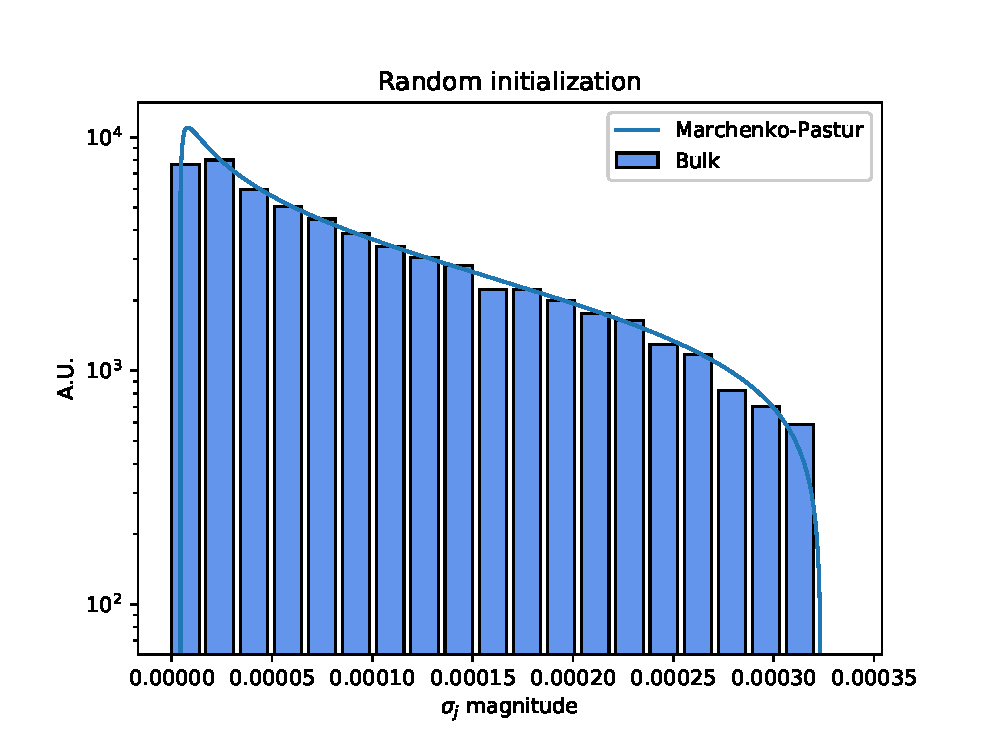
\includegraphics[width=\linewidth]{mp_fit.eps}
    \caption{}
    \label{fig:mp_fit}
  \end{subfigure}
  \begin{subfigure}{.32\linewidth}
    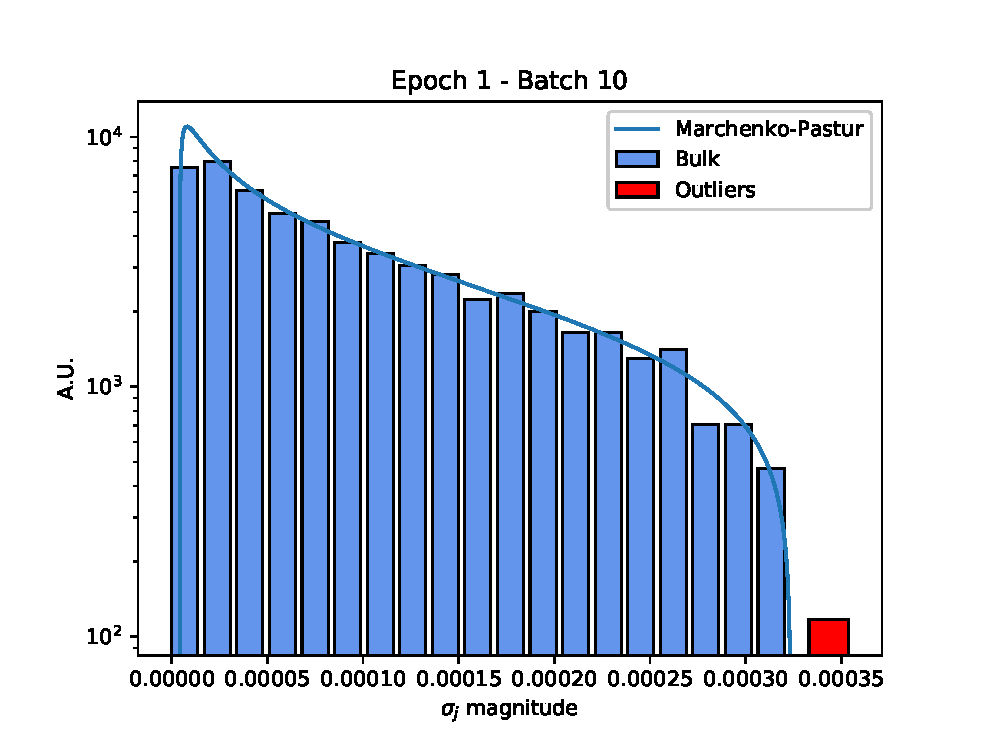
\includegraphics[width=\linewidth]{sv_distr_e1_b10.eps}
    \caption{}
    \label{fig:sv1}
  \end{subfigure}
  \begin{subfigure}{.32\linewidth}
    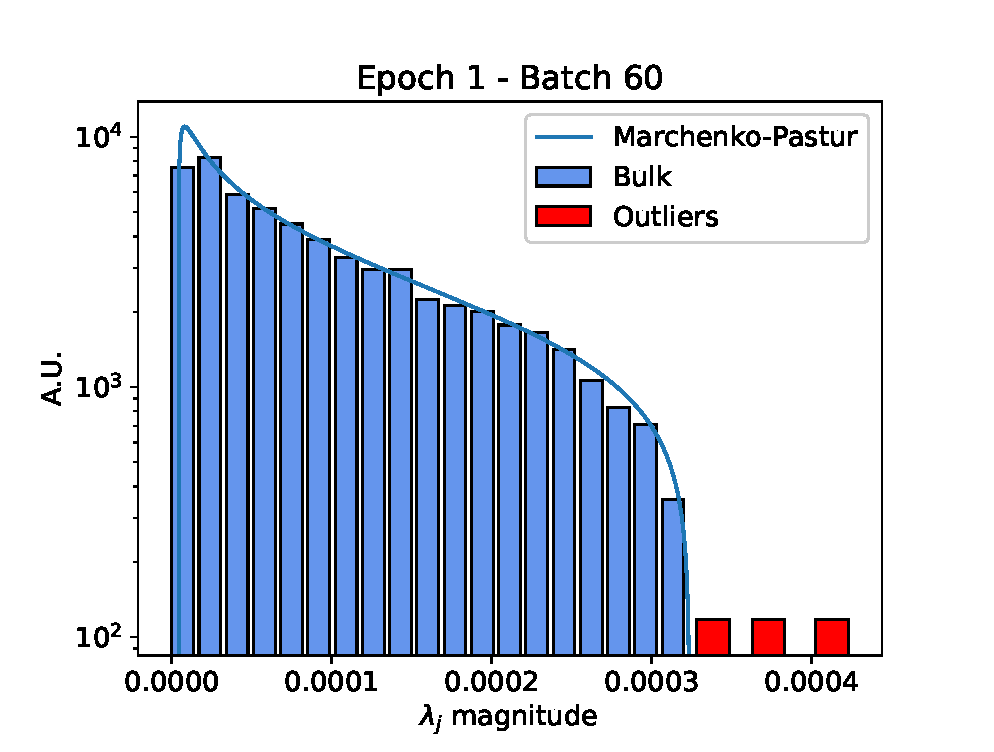
\includegraphics[width=\linewidth]{sv_distr_e1_b60.eps}
    \caption{}
    \label{fig:sv2}
  \end{subfigure}\par\medskip
  \begin{subfigure}{.32\linewidth}
    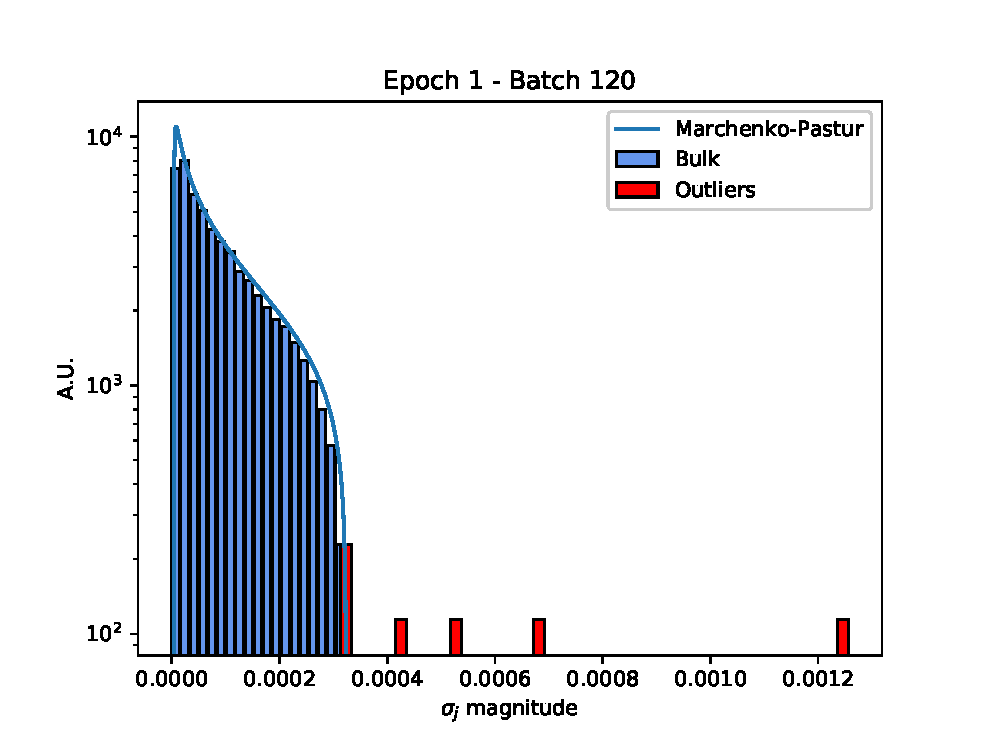
\includegraphics[width=\linewidth]{sv_distr_e1_b120.eps}
    \caption{} 
    \label{fig:sv3}
  \end{subfigure}
  \begin{subfigure}{.64\linewidth}
    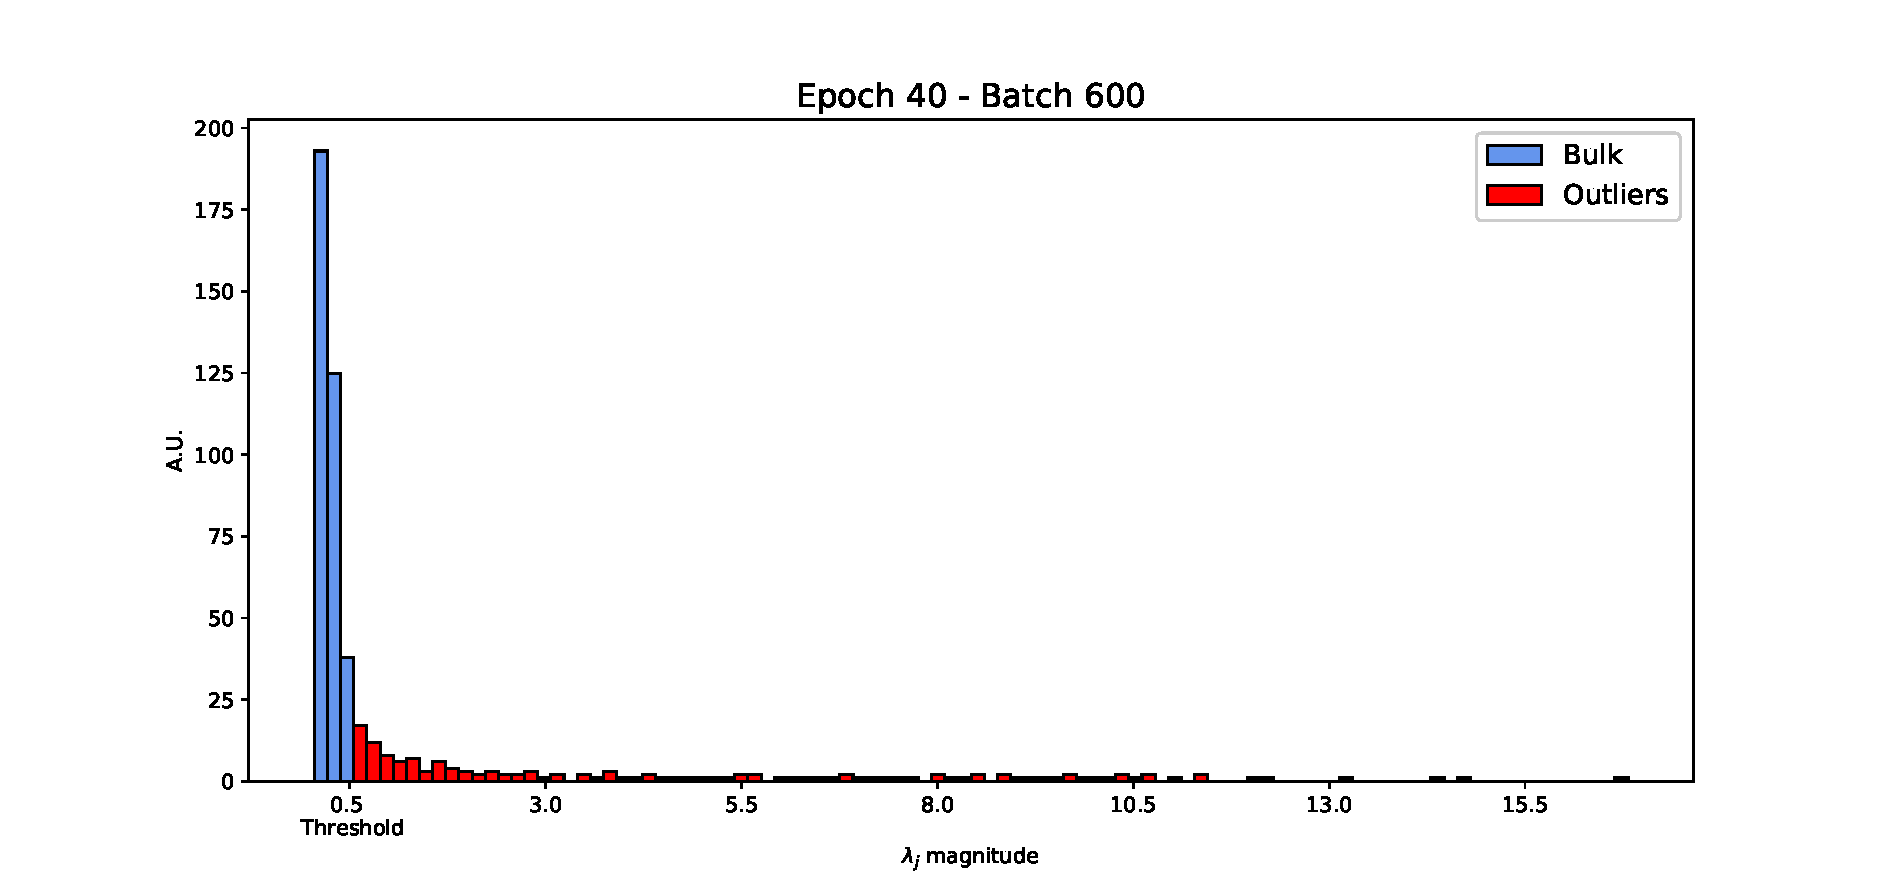
\includegraphics[width=\linewidth]{sv_distr_e40_b600.eps}
    \caption{}  
    \label{fig:sv4}
  \end{subfigure}
 \caption{\textbf{(a)} Singular values distribution of the initial random matrix compared to Marchenko-Pastur law. \textbf{(b)-(d)} With the training we can see some singular values strengthening and overcoming the threshold set by the Marchenko-Pastur law. \textbf{(e)} Distribution of the singular values after a long training: we can see many outliers spread above threshold and a spike of below-threshold singular values near zero.}
\end{figure}

Starting with the training we see that many singular values increase in magnitude and overcome the threshold for a gaussian random matrix; these are \textit{outliers} leaving the bulk, shown in fig. \ref{fig:sv1}-\ref{fig:sv3}. During the first epochs of the training this process is very fast and many \(\sigma_j\) are easily extracted from the bulk, growing of many orders of magnitude. The bulk is instead shrinked to low values, meaning that the \(\sigma_j\) that do not overcome the threshold decrease in magnitude. Going on with the training this process slows down but it does not stop: outliers keep growing slowly and the bulk keeps shrinking to approach a spike around zero. It is important to note that a kind of hierarchy is maintained in the process: the first outliers are never overcome by the newly extracted \(\sigma_j\), and this is made clear by looking at the corresponding left singular vectors (see next section).
After a long training the singular values \(\sigma_j\) are separated into two categories: a concentrated set of almost-null singular values and a set of outliers spread above the threshold, as shown in fig. \ref{fig:sv4}.

The evolution of the \(\sigma_j\) distribution described above suggests that the training process is able to discern between the \textit{most important} singular vectors, that are brought above threshold first and heavily strengthen, and a bulk of \textit{less important} singular vectors, that end up above threshold but whose \( \sigma_j\) reach values order of magnitude smaller then those of the strongest singular vectors. Moreover, the below-threshold singular vectors are practically eliminated by cutting down the corresponding \(\sigma_j\).

These observations give a good indication about what are the dynamics of the learning process, but there are some matters that need to be addressed: (i) it is not clear what singular vectors actually represent, (ii) the meaning of \textit{more} and \textit{less} important singular vectors has to be specified, (iii) no clues about stopping criteria for the learning are given.

\subsection{Analysis of left singular vectors}

To understand the role of the left singular vectors of a RBM we must keep in mind the interpretation for the SVD decomposition of \textbf{W} given previously. We have seen how the matrix of the weights \textbf{\(\Sigma\)} is shaped during the learning, and we recall that \textbf{V} is interpreted as a rotation in the space of the hidden units. We then expect to recover the structure of the training data into the \textbf{U} matrix, and to show this we carefully analyze the left singular vectors during training by visualizing them in the pixel space.

Before focusing on the left singular vectors, we note that also the external visible field can be visualized in the pixel space. With the initialization rule \eqref{eq:bias_init} we are able to encode into the field the mean activation of the visible layer, which is clearly shown in fig. \ref{fig:vbias} in the pixel space. If we instead initialize the visible field with a null vector, the mean activation pattern is learnt very effectively as the strongest left singular vector. The striking resemblance between the mean activation pattern computed from the training data and the one learnt by the RBM is shown in fig. \ref{fig:m1tr}-\ref{fig:vbias} and it serves as a first example of what the left singular vectors represent. It seems then equivalent to either encode the mean activation pattern into the visible field since the beginning or letting the RBM learn such a pattern as a left singular vector. In practice the second case is not desirable as the RBM associates to the mean activation pattern a very strong singular value, many orders of magnitude higher then the strongest outliers. This results in a bias in the sampling from the trained machine, such that the samples whose activation pattern is nearest to the mean are sampled with a higher frequency (in the worst case those are the only configurations sampled at equilibrium).

\begin{figure}
  \centering
  \begin{subfigure}{.15\linewidth}
    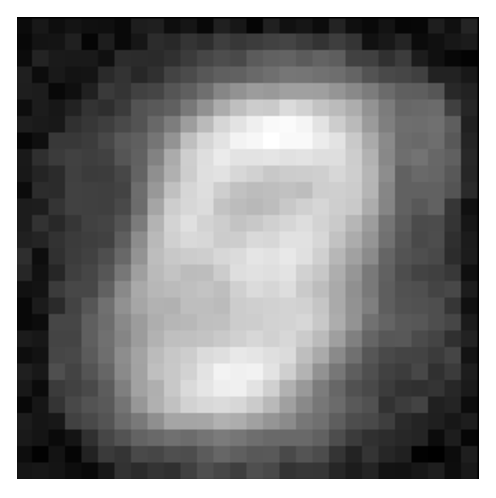
\includegraphics[width=\linewidth]{mode_1_training.eps}
    \caption{}
    \label{fig:m1tr}
  \end{subfigure}
  \begin{subfigure}{.15\linewidth}
    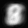
\includegraphics[width=\linewidth]{vbias.png}
    \caption{}
    \label{fig:vbias}
  \end{subfigure}
  \begin{subfigure}{.15\linewidth}
    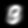
\includegraphics[width=\linewidth]{X_l_eigv_1.png}
    \caption{}
    \label{fig:m1data}
  \end{subfigure}\par\medskip
  \begin{subfigure}{\linewidth}
    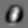
\includegraphics[width=.05\linewidth]{X_l_eigv_2.png}
    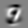
\includegraphics[width=.05\linewidth]{X_l_eigv_3.png}
    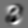
\includegraphics[width=.05\linewidth]{X_l_eigv_4.png}
    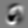
\includegraphics[width=.05\linewidth]{X_l_eigv_5.png}
    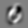
\includegraphics[width=.05\linewidth]{X_l_eigv_6.png}
    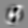
\includegraphics[width=.05\linewidth]{X_l_eigv_7.png}
    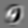
\includegraphics[width=.05\linewidth]{X_l_eigv_8.png}
    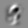
\includegraphics[width=.05\linewidth]{X_l_eigv_9.png}
    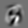
\includegraphics[width=.05\linewidth]{X_l_eigv_10.png}
    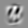
\includegraphics[width=.05\linewidth]{X_l_eigv_11.png}
    \caption{}
    \label{fig:modes_data}
  \end{subfigure}
  \begin{subfigure}{\linewidth}
    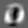
\includegraphics[width=.05\linewidth]{W_l_eigv_1.png}
    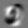
\includegraphics[width=.05\linewidth]{W_l_eigv_2.png}
    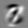
\includegraphics[width=.05\linewidth]{W_l_eigv_3.png}
    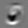
\includegraphics[width=.05\linewidth]{W_l_eigv_4.png}
    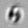
\includegraphics[width=.05\linewidth]{W_l_eigv_5.png}
    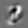
\includegraphics[width=.05\linewidth]{W_l_eigv_6.png}
    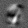
\includegraphics[width=.05\linewidth]{W_l_eigv_7.png}
    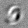
\includegraphics[width=.05\linewidth]{W_l_eigv_8.png}
    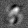
\includegraphics[width=.05\linewidth]{W_l_eigv_9.png}
    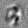
\includegraphics[width=.05\linewidth]{W_l_eigv_10.png}
    \caption{}
    \label{fig:modes_tr}
  \end{subfigure}\par
  \begin{subfigure}{\linewidth}
    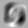
\includegraphics[width=.05\linewidth]{W_10_l_eigv_1.png}
    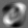
\includegraphics[width=.05\linewidth]{W_10_l_eigv_2.png}
    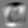
\includegraphics[width=.05\linewidth]{W_10_l_eigv_3.png}
    
\includegraphics[width=.05\linewidth]{W_10_l_eigv_4.png}
    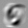
\includegraphics[width=.05\linewidth]{W_10_l_eigv_5.png}
    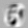
\includegraphics[width=.05\linewidth]{W_10_l_eigv_6.png}
    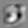
\includegraphics[width=.05\linewidth]{W_10_l_eigv_7.png}
    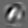
\includegraphics[width=.05\linewidth]{W_10_l_eigv_8.png}
    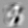
\includegraphics[width=.05\linewidth]{W_10_l_eigv_9.png}
    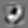
\includegraphics[width=.05\linewidth]{W_10_l_eigv_10.png}
    \caption{}
    \label{fig:modes_tr_10}
  \end{subfigure}
   \caption{\textbf{(a)} First mode learnt by the RBM with the external visible field initialized as a null vector. \textbf{(b)} External visible field initialized with rule \eqref{eq:bias_init}. \textbf{(c)} First principal components extracted from the training set. \textbf{(d)} Principal components extracted from the training set (starting from the second). \textbf{(e)} The first 10 modes of a RBM trained for 1 epoch, using initialization rule \eqref{eq:bias_init}. \textbf{(f)} Same as (e) but after a 10 epochs training.}
\end{figure}

The first 10 left singular vectors of a trained RBM are shown in fig. \ref{fig:modes_tr}-\ref{fig:modes_tr_10}. They are all composed by a homogeneous background on the borders and a set of alternating dark and light traits in the center, highlighting the fact that each singular vector acts globally on the visible layer. Even if the pictures seen in fig. \ref{fig:modes_tr}-\ref{fig:modes_tr_10} are quite different one from another, an interesting trend is found: a higher number of alternating traits is present in the successive vectors. At this point it is useful to draw a comparison to the Fourier decomposition of an image and interpret the left singular values as the \textit{modes} composing the activation pattern. The first singular vectors, characterized by a small number of alternating traits, play the role of the \textit{low frequency} modes while the successive modes act as \textit{high frequency} modes. The analogy to Fourier modes is suggested by the fact that we are basically performing PCA over the matrix \textbf{W} and the left singular vectors can be identified with the principal modes of variation (see \ref{sec:svd_pca}).

Looking at the dynamics of the learning it is seen that the modes take shape one by one as the corresponding singular value \(\sigma_j\) is brought above threshold. The subsequent strengthening of the \(\sigma_j\) corresponds to refinements and rotations, with little effects on the characterization of the modes as high or low frequency modes. For what concerns the modes below threshold, they present a dark border and a random configuration in the center; in this case the only effect of the training is to discern what are the units which are never activated and no information about the actual structure of the data is found.

These observations suggest that the RBM is able to learn the modes that compose the activation patterns of the data, starting with the low frequency modes and proceeding with the high frequency ones. Moreover, with reference to the \(\sigma_j\) distribution (fig. \ref{fig:sv4}), we note that the low frequency modes are given a higher weigth.

The dynamics described here and in the previous section present some similarities to the learning dynamics for deep linear neural networks \cite{ganguli}. Some insights on the behaviour of a RBM in the linear regime were given by looking at the SVD-like equations \eqref{eq:svd_like_vis}-\eqref{eq:svd_like_hid}, where we have seen how the magnetizations aligned to the strongest SVD modes are amplified. These magnetizations are thus unstable and they drive the formation of new mean-field fixed points during learning, that correspond to the magnetizations affine to the samples in the training set. These observations suggest a connection between the SVD of the data in the training set and the SVD of the weights matrix \(\mathbf{W}\), at least in the linear regime. This hypothesis is confirmed by comparing the SVD modes extracted from the data and those of the \(\mathbf{W}\) matrix, fig. \ref{fig:modes_data}-\ref{fig:modes_tr}, that are very similar. Going on with the training we expect non-linear effects to kick-in and this is seen in fig. \ref{fig:modes_tr_10} where the SVD of the data is not comparable to the SVD of \(\mathbf{W}\) anymore.

Summarizing, the analysis of the left singular vectors gives many insights on the training procedure:

\begin{itemize}
\item a RBM is able to learn the modes that compose the activation patterns of the training data
\item the low frequency modes are learnt first and are given higher weigths
\item at the beginning of the training the RBM operates in the linear regime and the \(\mathbf{W}\) matrix is shaped according to the SVD of the data in the training set
\item by continuing the training, new modes at increasing higher frequency are learnt while the already learnt modes are strengthen
\item the external visible field is equivalent to a left singular vector but we can avoid to learn it by using the appropriate initial conditions
\end{itemize}

\section{Characterization of the modes}
By looking at the singular values distribution of \(\mathbf{W}\) we have seen that there seem to be \textit{more} and \textit{less important} singular vectors. In the previous section we have then refined this observation by highlighting how the lowest-frequency modes are given the highest weights. We can then identify the more (less) important modes as the low (high) frequency ones. To gain some intuition about the meaning of this separation we can take our analogy further and think about the Fourier decomposition of a square wave; in such a case, the superposition of the low frequency harmonics is sufficient to build a good approximation of a square wave, while the role of the high frequency harmonics is that of sharpening the waveform at the discontinuity points. In the context of a trained RBM, we then expect that good approximations to the training data are obtained by exploiting only the low frequency modes, while the high frequency modes should represent minor corrections.

\begin{figure}
  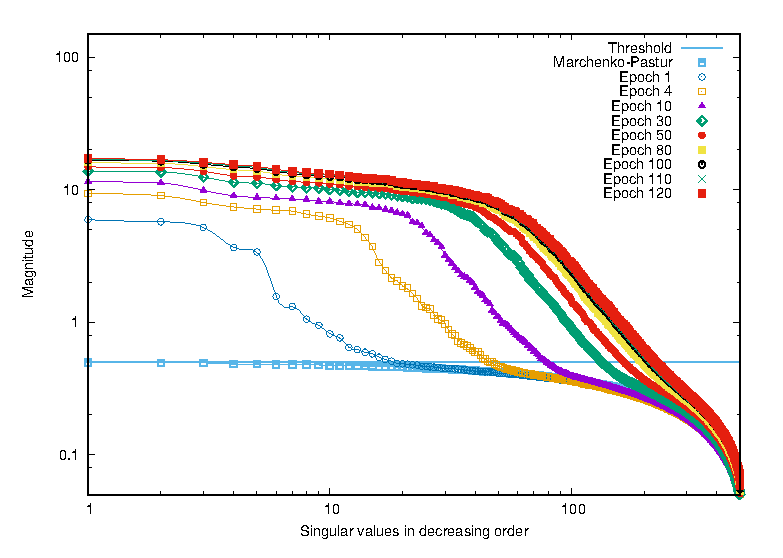
\includegraphics{SV_pl.eps}
  \caption{Log-log plot of the singular values represented as discrete asbscissas (in decreasing order) with their magnitude reported on the ordinates. A cutoff is highlighted by the onset of the linear behaviour.}
  \label{fig:sv_pl}
\end{figure}

It is not clear, however, how we can discern between high and low frequency modes. Some hints to address this issue are given by looking at the value of the \(\sigma_j\) in decreasing order on a log-log plot (fig. \ref{fig:sv_pl}), in which an interesting picture emerges: the strongest \(\sigma_j\) are located far above threshold and are of comparable magnitude, followed by a tail of exponentially damped \(\sigma_j\). This picture is consistent across the training, the only difference being the damping cutoff that is increasing with the epochs. After a long training, however, the increase in the cutoff is very slow and this could serve as a signal to stop the learning, as such situation amounts to slowly strengthening singular values which are exponentially less important then the already learnt modes.

We are then driven to define the more important low frequency modes as the modes before cutoff, and the exponentially less important high frequency modes as those after cutoff. A consistency check is shown in fig. \ref{fig:hf_modes}, where just the 100 strongest modes are retained to construct the samples and the remaining modes are shown to encode boundary corrections. Choosing the first 100 modes is arbitrary; in fig. \ref{fig:sv_pl} we can see how the cutoff is well below 100, so with this choice we are sure that we included in the reconstruction of the samples all the strong modes before cutoff plus a small number of modes giving boundary corrections.

As a conclusion, the above observations suggest that the weights matrix of a trained RBM is composed by two classes of modes; recalling the expansion \eqref{eq:w_exp} we can express the components of \(\mathbf{W}\) as

\begin{equation}
w_{ij} = \sum_{\alpha \in bulk} \sigma_{\alpha} u_{i,\alpha} v_{j,\alpha} + \sum_{\alpha \in outliers} \sigma_{\alpha} u_{i,\alpha} v_{j,\alpha}
\label{eq:params_exp}
\end{equation}

where the modes of the bulk are those that remain random after the training (below threshold or after cutoff) while the outliers correspond to the modes that actually encode the structure of training data. The proposed form for \(\mathbf{W}\) suggests that the statistical properties of the outliers are those important for determining the proper statistical ensemble of the RBM model; this could make it possible to theoretically analyse realistic RBM neural networks with the tools of statistical physics, improving current attempts relying on unrealistic approximations \cite{monasson}.

\begin{figure}
  \begin{subfigure}{\linewidth}
  	\centering
    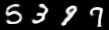
\includegraphics[width=.4\linewidth]{complete40ep.png}
    \caption{}
  \end{subfigure}\par
  \begin{subfigure}{\linewidth}
  	\centering
    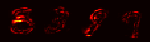
\includegraphics[width=.4\linewidth]{difference20ep.png}
    \caption{}  
  \end{subfigure}\par
  \begin{subfigure}{\linewidth}
  	\centering
    \includegraphics[width=.4\linewidth]{difference40ep.png}
    \caption{}
  \end{subfigure}
  \caption{\textbf{(a)} The image shows some samples obtained with the trained RBM (after a 40 epochs training) and then "filtered" by eliminating the 400 weakest modes (just the 100 strongest modes are retained). \textbf{(b)} The images are composed by eliminating the 100 strongest modes to see what the weakest modes actually encode (20 epochs training). \textbf{(c)} As in \textbf{(b)} but after a 40 epochs training.}
  \label{fig:hf_modes}
\end{figure}

\section{Conclusion}

The analisys of the learning dynamics of a RBM led to a better understanding of how this elementary generative model is working, and how the structure of training data is dinamically learnt. 

The first step in our work has been to compare the new physics-inspired EMF training algorithm to the PCD algorithm classically used to train RBMs. Inspection of the samples generated by the model has shown how the PCD method is slightly preferable; this is probably related to the fact that the training has been observed to increase the inverse effective temperature of the RBM, which is defined as the variance of the weights distribution. The weak couplings expansion on which EMF relies is then justified at the beginning of the training, but it breaks down after a small number of training epochs (less then \(20\) in our case, as we have seen the effective temperature to converge to a stable value after about \(20\) epochs). For all the other aspects of our investigation, however, no difference is found between PCD and EMF, showing how the learning dynamics are instrinsically related to the definition of the RBM model itself and independent on the training procedure.

The behaviour of the inverse temperature also suggests that the training of a RBM is initially operated in the linear regime. In this learning phase, the mean-field approximation borrowed from statistical physics has proved to be a valuable investigation tool. In fact, linearization of mean-field equations provided the new SVD-like equations \eqref{eq:svd_like_vis}-\eqref{eq:svd_like_hid} that show how the SVD of the weights matrix \(\mathbf{W}\) is linked to the SVD of the training data. This link has been proven experimentally by tracking the evolution of the left singular vectors of the \(\mathbf{W}\) matrix, interpreted as the modes composing the generated models. Those have been found to approximate very well the corresponding principal components of the training data during the first epochs of the training, while for later epochs non-linear effects kick in and the similarity is lost.

Beyond the linear regime, the evolution of the singular values highlights a more comprehensive description of the learning procedure as a whole. We have seen how the singular values and the corresponding singular vectors are learnt one by one quite fast, and they are then strengthen by proceeding the training. This process does not really come to an end, but it slows down significantly after many epochs revealing a cutoff in the number of learnt modes. We believe this is an important observation suggesting that an indicator defined on the learnt modes could eventually signal the end of the learning, providing a rigorous stopping criterium.

The investigation presented in this report serves as a first step in the determination of the statistical properties of trained RBMs. The emerging picture is that parameters of the model are in part random (interpreted as noise) and in part structured and related to data. This is expressed in eq. \eqref{eq:params_exp}, where the set of outliers is the one of interest; determining the statistical properties of this subset of parameters (starting with mean and variance, to proceed by determining the form of the distribution) would lead to the association of a proper statistical ensemble to the RBM model, improving on current approximations based on unrealistic assumptions such as independence of the weights \cite{monasson}.

Altogether, our analysis of the learning dynamics helped shading some lights on the inner workings of the RBM model, providing a useful framework in which subsequent investigations can more easily be performed.

\begin{acknowledgements}
This work has been done under the supervision of C. Furtlehner and A. Decelle. Fruitful discussions with C. Leroy, who has been working in the same team on a related topic, have also been of help developing the subject.
\end{acknowledgements}

\begin{thebibliography}{9}

\bibitem{go}
D. Silver et al., "Mastering the game of Go with deep neural networks and tree search",
\textit{Nature}, 529, p. 484–489, 2016.

\bibitem{foundations}
F. Cucker, S. Smale, "On the mathematical foundations of learning",
\textit{Bull. Amer. Math. Soc.}, 39, p. 1-49, 2002.

\bibitem{hist1}
W. Krauth, M. Mezard, "Machine Learning algorithms with optimal stability in neural networks",
\textit{Journal of Physics A: Mathematical and General}, 20, L745–L752, 1987.

\bibitem{hist2}
J. J. Hopfield, "Neural networks and physical systems with emergent collective computational abilities"\textit{Proceedings of the National Academy of Sciences, 79}, 8, p. 2554–2558, 1982.

\bibitem{tap_train}
M. Gabri\'e, E. W. Tramel, F. Krzakala,
Training Restricted Boltzmann Machines via the Thouless-Anderson-Palmer Free Energy,
\textit{Advances in Neural Information Processing Systems (NIPS)}, 28, pages 640--648, 2015.

\bibitem{tap}
E. W. Tramel, M. Gabri\'e, A. Manoel, F. Caltagirone, F. Krzakala, \textit{arXiv:1702.03260}

\bibitem{monasson}
J. Tubiana, R. Monasson, "Emergence of Compositional Representations in Restricted Boltzmann Machines",
\textit{Phys. Rev. Lett. 118, 138301}, 2017.

\bibitem{Hinton_CD}
G. E. Hinton, “Training products of experts by minimizing Contrastive divergence,”
\textit{Neural computation}
, vol. 14, pp. 1771-1800, 2002.

\bibitem{PCD}
T. Tieleman, “Training restricted Boltzmann machines using approximations to the likelihood gradient,”
\textit{ICML}, Vol. 307, p. 7, 2008.

\bibitem{Hinton_guide}
G. E. Hinton, "A Practical Guide to Training Restricted Boltzmann Machines", \textit{Proceedings of Neural Networks: Tricks of the Trade (2nd ed.)}, pages 599-619, 2012. 

\bibitem{PCA}
I.T. Jolliffe, "Principal Component Analysis",
\textit{Springer-Verlag New York}, 2002.

\bibitem{SK}
D. Sherrington, S. Kirkpatrick,
"Solvable Model of a Spin-Glass",
\textit{Phys. Rev. Lett.}, Vol. 35, 1975.

\bibitem{ht_exp}
A. Georges, J. S. Yedidia,
"How to expand around mean-field theory using high-temperature expansions",
\textit{Journal of Physics A: Mathematical and General}, Volume 24, Number 9, 1991

\bibitem{TAP}
D. J. Thouless , P. W. Anderson, R. G. Palmer,
"Solution of 'Solvable model of a spin glass'",
\textit{Philosophical Magazine}, Vol. 35:3, p. 593-601, 1977

\bibitem{conv}
E. Bolthausen, "An Iterative Construction of Solutions of the TAP Equations for the Sherrington–Kirkpatrick Model", \textit{Commun. Math. Phys.}, Vol. 325, pages 333-366, 2014.

\bibitem{mnist}
http://yann.lecun.com/exdb/mnist/

\bibitem{gibbs}
G. Casella and E. I. George, "Explaining the Gibbs Sampler",
\textit{The American Statistician},
Vol. 46, No. 3, pp. 167-174, 1992.

\bibitem{leroy}
C. Leroy made an investigation on TAP fixed points and free energy landscape while at Laboratoire de Recherche en Informatique, working in my same team.

\bibitem{Nishimori}
H. Nishimori, "Statistical Physics of Spin Glasses and Information Processing: An Introduction",
\textit{Oxford University Press}, 2001

\bibitem{MP_law}
Marchenko, V.A. and Pastur, L.A., "Distribution of Eigenvalues for Some Sets of Random Matrices", \textit{Sbornik: Mathematics}, Vol. 1, pages 457-483, 1967.

\bibitem{ganguli}
A. M. Saxe, J. L. McClelland, S. Ganguli, "Exact solutions to the nonlinear dynamics of learning in deep linear neural networks",
\textit{arXiv:1312.6120}, 2014.

\end{thebibliography}


\appendix*

\section{Learning dynamics in the linear regime}
A more detailed description of the relation between the SVD of the data and that of the weights matrix can be given. To do that, we define a deterministic dynamics for the learning equations \eqref{eq:w_up}, \eqref{eq:a_up}, \eqref{eq:b_up} and show how at equilibrium they drive the learning of the strongest SVD modes of the data. Introducing a time variable \(t\) we rewrite \eqref{eq:w_exp} as

\begin{equation}
\label{eq:w_t}
w_{ij}(t) = \sum_{\alpha} \sigma_{\alpha}(t) \mu_{i,\alpha}(t) \nu_{j,\alpha}(t)
\end{equation}

and we take the continuous limit of the learning equations to obtain

\begin{align}
\label{eq:cont1}
\frac{dw_{ij}}{dt} & = \langle v_i h_j \rangle_{data} - \langle v_i h_j \rangle_{model} \\
\label{eq:cont2}
\frac{d a_i}{dt} & = \langle v_i \rangle_{data} - \langle v_i \rangle_{model} \\
\label{eq:cont3}
\frac{d b_j}{dt} & = \langle h_j \rangle_{data} - \langle h_j \rangle_{model}
\end{align}

The left hand side of \eqref{eq:cont1} can be expressed in a simple form by expanding it over the basis defined by the SVD and exploiting \eqref{eq:w_t}

\begin{align}
\label{eq:w_svd_exp}
\left( \frac{d \mathbf{W}}{dt} \right)_{\alpha \beta} & = \sum_{ij} \mathbf{\mu}_{i,\alpha} \frac{d w_{ij}}{dt} \mathbf{\nu}_{j,\beta} \nonumber \\
& = \delta_{\alpha, \beta} \frac{d \sigma_{\alpha}}{dt} + (1 - \delta_{\alpha \beta} ) \left( \sigma_{\alpha} \frac{d \mathbf{\nu}_{\alpha}^T}{dt} \mathfb{\nu}_{\beta} + \sigma_{\beta} \mathbf{\mu}_{\alpha}^T \frac{d \mathbf{\mu}_{\beta}}{dt} \right) \nonumber \\
& = \delta_{\alpha, \beta} \frac{d \sigma_{\alpha}}{dt} + (1 - \delta_{\alpha \beta} ) \left( \sigma_{\alpha} \Omega_{\alpha \beta}^h + \sigma_{\beta} \Omega_{\beta \alpha}^v \right)
\end{align}

where we have defined the generators of rotations in both \(\mathbf{\mu}_{\alpha}\) and \( \mathbf{\nu}_{\alpha}\) bases

\begin{align}
\label{eq:Omega_ref_v}
\Omega_{\alpha \beta}^v(t) & = \frac{d \mathbf{\mu}_{\alpha}^T}{dt} \mathbf{\mu}_{\beta} \\
\label{eq:Omega_ref_h}
\Omega_{\alpha \beta}^h(t) & = \frac{d \mathbf{\nu}_{\alpha}^T}{dt} \mathbf{\nu}_{\beta}
\end{align}

This let us see how off-diagonal variations are related to the basis rotations, while the diagonal dynamics correspond to eigenvalues changes.
% Introducing the symmetric and antisymmetric parts of \( \frac{d \mathbf{W}}{dt} \) we can rewrite definitions \eqref{eq:Omega_def_v},\eqref{eq:Omega_def_h} as

%\begin{align}
%\Omega_{\alpha \beta}^v = \frac{2}{\sigma_{\alpha} + \sigma_{\beta}} \left( \frac{d \mathbf{W}}{dt} \right)_{\alpha \beta}^A - \frac{2}{\sigma_{\alpha} - \sigma_{\beta}} \left( \frac{d \mathbf{W}}{dt} \right)_{\alpha \beta}^S \\
%\Omega_{\alpha \beta}^h = \frac{2}{\sigma_{\alpha} + \sigma_{\beta}} \left( \frac{d \mathbf{W}}{dt} \right)_{\alpha \beta}^A + \frac{2}{\sigma_{\alpha} - \sigma_{\beta}} \left( \frac{d \mathbf{W}}{dt} \right)_{\alpha \beta}^S
%\end{align}

Projecting the full learning equations on the SVD basis we obtain

\begin{align}
\label{eq:cd_svd_w}
\left( \frac{d \mathbf{W}}{dt} \right)_{\alpha \beta} & = \langle v_{\alpha} h_{\beta} \rangle_{data} - \langle v_{\alpha} h_{\beta} \rangle_{model} \\
\left( \frac{d \mathbf{a}}{dt} \right)_{\alpha} & = \langle v_{\alpha} \rangle_{data} - \langle v_{\alpha} \rangle_{model} \\
\left( \frac{d \mathbf{b}}{dt} \right)_{\alpha} & = \langle h_{\alpha} \rangle_{data} - \langle h_{\alpha} \rangle_{model}
\end{align}

with

\begin{equation}
v_{\alpha} = \sum_i v_i \mu_{i,\alpha} \, , \qquad h_{\alpha} = \sum_j h_j \nu_{j,\alpha}
\end{equation}

In order to proceed, we consider the expansion to second order of the mean-field free energy

\begin{align}
F(\mathbf{m}^v,\mathbf{m}^h) & = \frac{1}{2} \sum_{i = 1}^N (1 + m_i^v) \log (1 + m_i^v) + (1 - m_i^v) \log (1 - m_i^v) \\
& + \frac{1}{2} \sum_{j=1}^M (1 + m_j^h) \log (1 + m_j^h) + (1 - m_j^h) \log (1 - m_j^h) \\
& - \sum_{i,j} w_{ij} m_i^v m_j^h + \sum_{i=1}^N a_i m_i^v + \sum_{j=1}^M b_j m_j^h \\
& \simeq \frac{1}{2} \sum_{i=1}^N \left(m_i^v\right)^2 + \frac{1}{2} \sum_{j=1}^M \left(m_j^h\right)^2 - \sum_{ij} w_{ij} m_i^v m_j^h + \sum_{i=1}^N a_i m_i^v + \sum_{j=1}^M b_j m_j^h
\end{align}

The corresponding probability measure is Gaussian, for which we can write the covariance matrix in the following form (\(\sigma_v, \sigma_h\) being the variances of visible and hidden magnetizations)

\begin{equation}
\operatorname{cov}(\mathbf{m^v},\mathbf{m^h}) =
\begin{pmatrix}
\frac{\sigma_h^{-2}}{\sigma_v^{-2} \sigma_h^{-2} - \mathbf{W W^T}} & {\mathbf{W}\frac{1}{\sigma_v^{-2} \sigma_h^{-2} - \mathbf{W^T W}} \\
\mathbf{W^T} \frac{1}{\sigma_v^{-2} \sigma_h^{-2} - \mathbf{W W^T}} & \frac{\sigma_h^{-2}}{\sigma_v^{-2} \sigma_h^{-2} - \mathbf{W W^T}} 
\end{pmatrix}
\end{equation}

In this mean-field picture, the values of visible and hidden nodes are identified with the magnetizations. This consists in treating a RBM with Gaussian variables and further assuming the external fields and the mean of the data to be null (normalization and rescaling of the training set can determine such conditions) we can rewrite the empirical expectation in \eqref{eq:cd_svd_w} as

\begin{equation}
\langle v_{\alpha} h_{\beta} \rangle_{data} = \sigma_h^2 \sigma_{\beta} \langle v_{\alpha} v_{\beta} \rangle_{data} = \sigma_h^2 \sigma_{\beta} \operatorname{cov}(v_{\alpha}, v_{\beta})
\end{equation}

where we see that the covariance matrix of the data comes out. Plugging the above equation into \eqref{eq:cd_svd_w} and recognizing also the average over the model as a covariance, the diagonalized equation that we obtain defines the evolution of the singular values

\begin{equation}
\frac{d \sigma_{\alpha}}{dt} = \sigma_h^2 \sigma_{\alpha} \left( \langle v_{\alpha}^2 \rangle_{data} - \frac{\sigma_v^2}{1 - \sigma_v^2 \sigma_h^2 \sigma_{\alpha}^2} \right)
\end{equation}

By linear analysis we can find the stable fixed points for the above equation, given by

\begin{equation}
\sigma_{\alpha}^2 =
\begin{cases}
\frac{\langle v_{\alpha}^2 \rangle_{data} - \sigma_{v}^2}{\sigma_{v}^2 \sigma_{h}^2 \langle v_{\alpha}^2 \rangle_{data}} & \langle v_{\alpha}^2 \rangle_{data} > \sigma_v^2 \\
0 & \langle v_{\alpha}^2 \rangle_{data} < \sigma_v^2 
\end{cases}
\end{equation}

and we see how the evolution of the singular values in the linear regime is driven by the SVD modes of the training data. The strongest modes, those above the threshold \( \sigma_v^2 \), are selected and learnt while the modes below threshold are damped.

\end{document}
